\chapter{Business Information Visualization of time-oriented Data}
\label{chap:BIV}


\iffalse
\listoftodos

\section{Outline} \todo{Remove from BA}
\begin{enumerate}
    \item The role of InfoVis in Business. Visual Analytics. Selfservice. Insights in Company/ Business. $\Rightarrow$ Business Data
    \subitem But: Other data types also in Business: IoT. Not covered because it is a too wide topic.
    \subitem Business use VA tools to get insight into data.
    \item Need for good visualizations for Business data
    \subitem What are business data? $\Rightarrow$ data types
    \item 2nd challenge: BigData.
    \subitem Where does BigData occur? Application Areas. Streaming Data
    \subitem Is BigData relevant for Business Data? Application Areas of Business Data
    \item Solutions in Literature
    \subitem Aggregation
    \subitem Abstraction
    \item Tools in Business
    \subitem Requirements: Visual Analytics Tools
    \subitem New Visualization Techniques -> Extensionability (p.12, "open
framework fed with pluggable visual and analytical components for analyzing
time-oriented data is useful. Such a framework will be able to support multiple
analysis tasks and data characteristics, which is a goal of Visual Analytics."
\cite{Aigner2007})
    \subitem Market Relevance: Qlik, Tableau
    \subitem Other Approaches: Jaspersoft(because its scalable),
    \subitem Comparison
    \item Conclusion: Which tool for time-oriented data?
\end{enumerate}
\fi
----- \\*
% Business Information Visualization
\section{The Role of Visualization in Business} \label{BIV}
Tools for Business Intelligence (BI) and Analytics, visualization, data discovery as well as for data mining continually gain importance in companies to assist humans to gain insights into their data. Although the differentiation between those tools is not selective and the terms are not clearly distinguished we can make the following differentiation: Data Mining tools allow automatic decision-making by applying algorithms to the data and extract patterns in an automatic way\cite{Goebel1999} while exploratory data analysis (EDA) tools are used to mine data with support of human input. We will use the definition of EDA tools if we speak of visualization tools in this work. As a pwc-survey showed eventhough automatic ways for decision support exists data analysis stil relies on human judgement and thus\cite{PwC2016}, visualization tools are used to support the business user in the data discovery process.

Decision-maker usually are part of the management domain and thus, come from the marketing, sales or management-field but the majority of them uses these tools with few computer science background. Therefore, tools have to be self-explaining, easy-to-use \cite{Crapo2000} and without the requirement of extensive programming. Especially visualization plays an important role as it reduces the information overload\cite{Keima} and simplifys the process of problem-solving\cite{Zhang}. Eventhough we only consider visualization tools which are used to explore data visualization tools have the two roles of presentation and exploration\cite{Crapo2000}. Visualization as presentation is either used to display data without any data mining algorithm or visualization as presentation is used to present the results of a data mining algorithm. Visualization as exploration is used before and during the data mining algorithm to explore the data interactively. This group is called visual analytics. The decision-maker needs both processes for decision making as results are presented on the screen and to explore the data interactively\cite{Ware2012a}. 
Talking of visualization an important data type for business is time-oriented data(\ref{data}) as it allows business to analyze the past and predict the future of the company\cite{Ao2010}. We will have a closer look at user tasks in section \ref{tasks}.
 
\begin{figure}[H]
    \centering
        \scalebox{.5}{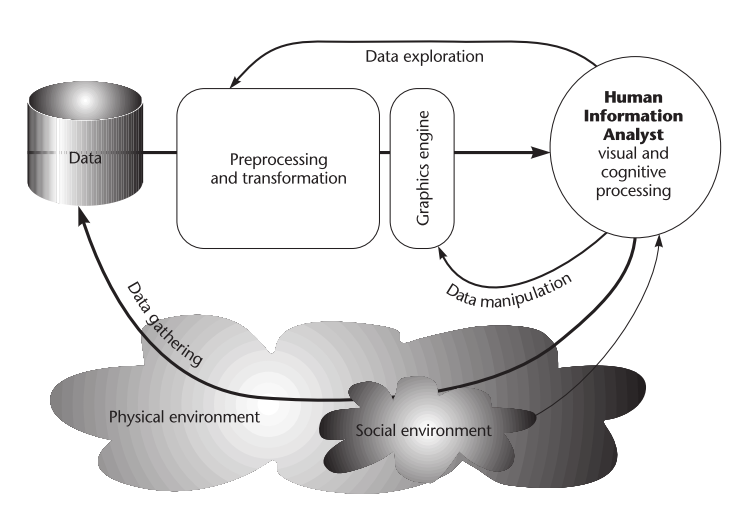
\includegraphics{src/images/VisPipeline}}
    \caption{Visualization Pipeline \cite{Ware2012a}}
    \label{fig:my_label}
\end{figure}

\section{Large Data}
Nowadays, the challenge in BIV is to handle large amounts of data and displaying them in an effective manner. The effective manner was defined by Shneiderman \cite{paterno1997concurtasktrees, Shneiderman2008, Keim2008}: \textit{"Overview first, zoom in and filter, then details on demand}. Overview is a basic yet important task because it navigates the user in the data and allows further analysis. But as large data appears with a number of challenges creating this overview is more difficult:
\\*
\textit{Overlap}: 
If the whole dataset is visualized or even a subset the data may overlap and reduce visual clutter.
\\*
\textit{Visual Noise}: 
Even if data items are not overlapping data in large datasets might be to similar to each other. Thus, the user cannot differentiate distinct items on the screen.
\\*
\textit{Limited monitor resolution}:
Even if large monitors are used to visualize data in the end the available pixels on the monitor is smaller than the number of data items in a dataset. 
\\*
\textit{Limited visual perception}:
Moreover, human perception is limited.
\\*
\textit{Information Loss}:
While reducing the number of data items to present them on the limited screen informations in the data can be lost. The important question is which data characteristics to keep such that the user tasks still can be supported.

This is why Shneiderman itself extended its own mantra with the use of aggregation markers and Keim formulated it as \textit{Analyze First - Show the Important - Zoom and Filter, and Analyze Further - Details on Demand}\cite{Keima}. The effective representation of large amounts of data requires to extend the Overview by the use of aggregation which can be achieved by appropriate techniques, correct parameterization, interaction and analytical methods\cite{Aigner2008}. 


% Users in BIV are usually no computer scientist. [Share of Workers in Business] 
% Self-Service Data
% Role of Visual driven analysis -> need for tools





\section{Definitions}
In order to give a clear impression of the used terms we define frequently used expressions.

\textbf{Information Visualization}\\*
Information Visualization is the graphical representation of non-spatial or abstract data\cite{Keim}. In contrast to scientific visualization the data which is visualized in information visualization does not have an inherent 2D or 3D structure\cite{Shneiderman2008}. 
As business data usually is abstract, discrete and multi-variate according to \cite{Tegarden1999} the type of visualization for business data is Information Visualization.

\textbf{Visualization technique}\\*
The way how data variables are mapped to graphical primitives is called visualization technique. Typical examples are bar charts, line charts or scatterplots. Thereby, every technique has its own philosophy how to present the data (called \textit{Visual Metaphor}\cite{Tegarden1999}), its own strengths and weaknesses and its particular application. Typically new visualization techniques are created for a specific application and the available amount of visualization technique is huge and continually growing. In this work we will focus on \textit{time-oriented data} and thus, only consider visualization techniques for this cause. Moreover, we will exclude visualization systems which are combined techniques. 
\\*

\textbf{Visual Data Exploration}\\*

\textbf{Time-oriented Data}\\*
Time-oriented data is data which is linked to time\cite{Aigner2011}. Often, time-oriented datasets are very large and multi-variate which makes it difficult to analyze them. The question is how time-oriented data can be analyzed if the number of data points exceeds the screen resolution. This brings us to the definition of large time-oriented Data. 
We define large time-oriented Data as abstract time-dependent data which is too large to fit on the screen. \cite{Shneiderman2008} 
In the following work, we will use time-oriented Data, time-oriented Big Data and Big time-oriented Data equivalently for large time-oriented Data. 




\textbf{Visualization Tools}\\*
While BI is defined as...\todo{Definition BI} data mining describes the extraction of patterns and models of the underlying data structure\cite{FerreiradeOliveira2003}. When data mining is used together with visualization data mining is based on automated algorithms which detect relevant patterns and display the results afterwards. In contrast, visual data exploration is a completely human guided process\cite{FerreiradeOliveira2003}. First data is displayed on the screen as a visualization and with the help of human visual capabilities new hypothesis are formed. Data visualization is a more general term for generating a graphical representation out of data and is used as well in BI, Analytics, data discovery as in visual analytics. 
Visualization tools display hundreds of items on the screen and offer interaction techniques such as zooming and filtering\cite{Shneiderman2008}.


% Data types for Information Visualization
\section{Data type} \label{data}

For choosing appropriate visualization techniques the first step is in understanding the underlying data and creating a correct data model\cite{Aigner2011}, so that the visualization technique represents the underlying data structure and offers best insights\cite{Bacic}. \textit{Aigner et. al.} proposed  the following questions to model the visualization problem: 
\begin{itemize}
    \item What is presented?
    \item Why is it presented?
    \item How it is presented?
\end{itemize}
\textbf{What is presented?}\\*
Talking of large time-oriented data for business we will consider the three given characteristics of the data: characteristics of business data, time-dependency and the size. Business data is collected in many different areas. The following table gives an overview about the applications: 

\begin{table}[th]
	\centering
	% caption format: \caption[<business aplications>]{<long version>}
	\caption[Table 1]{Business applications\cite{Brachman1996,Tegarden1999}}
	\label{businessapplications}
	\begin{tabu}{lcc}
	\toprule
	Marketing & Financial Sector \\
	Fraud Detection & Manufacturing and Production \\
	Operations Planning & Market Analysis \\
	Health Care & Network Management\\
	\bottomrule
	\end{tabu}
\end{table}

The bottom line is that business data ususally is abstract and multi-variate according to Tegarden\cite{tegarden1999}. Multi-variate data is usually presented in tables\cite{Borgo2013} and thus we assume that business data is given in tables, each attribute is represented by a column and each row is one data item. The attributes can be either numerical or text-based. 
Talking of time-oriented business data we assume that the data is linked to time. The time-dependency of the data structures the data by a given order. Every data item is mapped to a specific point in time with a smallest possible unit such as seconds. Time with a smallest unit is mapped to integer\cite{Aigner2011} and thus we assume that time-oriented business data is discrete and has a given order. Ordered discrete data is called \textit{time series}. The time series is an ordered sequence of n data items $T=(t_1+t_2+...+t_n),t_i\in\mathbb{R}$. Eventhough, data can be point-based or interval-based (scope), linear or cyclic (arrangement), ordered branching and with multiple perspectives(viewpoint)\cite{Aigner2011}. We will not narrow our focus further but talk on an abstract level. Our perpective is to explore visualization techniques with different scopes, arrangements and viewpoints according to their scalability but of course, every visualization technique is designed for a specific scope such as linearity or seasonal behaviour. The decision for a specific visualization technique is still up to the user. \todo{hier evtl. die unterscheidung von radial und nicht radial einführen / linear oder zyklisch?}.
Lastely, we will characterize the size of the data. We are considering large and huge amounts of data. Large data is defined according to\cite{Huber1994} as datasets with $10^6$ and huge data with $10^8$ data entries.


% User Tasks
\section{Time-oriented User Tasks} \label{tasks}
\textbf{Why is it presented?}\\*
Every tool for decision-support should consider the user perspective. The business user is a kind of person which is interested in verify existing hypothesis (verification) and discover new patterns (discovery) and by using the tool he expects the tool to assist him in analyzing the data, finding critical points and perform analysis automatically\cite{Brachman1996}. Verification and discovery in the analysis of time-oriented data can be split in seven major tasks\cite{Esling2012}:

\\*
\textbf{T1: Query by Content}\\*
Query by content describes the retrieval of similar items to the query and returns a set with the most similar solutions to the query. In time-oriented data query by content returns the \textit{k} most similar time series to the queried time series.
\\*
\textbf{T2: Clustering}\\*
Clustering is the process of finding expressive groups (clusters) out of the data. Therefore, the dataset is devided into subgroups according to some similarity measure. In the context of large time-oriented data clustering is important to compare similar time-series.
\\*
\textbf{T3: Classification}\\*
In classification the task is to find the right group the item belongs to. According to \textit{Aigner et al.} temporal classification describes the preprocess of finding the correct group for given data or dataset. This task is important for large data to abstract the data and make them handable. As this task is preprocessing and not data presentation or exploration we will not check whether the tools support the user in this task. 
\\*
\textbf{T4: Segmentation}\\*
Segmentation splits a time series into \textit{k} meaningful subsequences (segments)\cite{batyrshin2007perception}. 
\\*
\textbf{T5: Prediction}\\*
In Prediction\textit{k} future events are predicted based on the past \textit{n} time series. This process is also known as \textit{forecasting}. Forecasting 
\\*
\textbf{T6: Anomaly Detection} \\*
Anomaly detection points out events which behave in a different way than expected.
\\*
\textbf{T7: Pattern Discovery} \}\*
Pattern discovery finds regularly appearing structures in a time series.  It covers the exploration of trends, outliers and clusters. Especially, in business this task is one the most important tasks.\todo{quote finden}


\iffalse
\begin{tikzpicture}[sibling distance=12em,
  every node/.style = {shape=rectangle, 
    draw, align=center,
    top color=white}]]
  \node [shape = ellipse] {Visualization Tasks}
    child { node [shape = ellipse] {visualization methods} %time-oriented data: 
      child { node [shape = ellipse] {right visualization method} }
      child { node [shape = ellipse] {right parametrization} 
        child { node {navigation in time} }
        child { node {search} }
        child { node {comparison} }
        child { node {manipulation} } } }
    child { node [shape = ellipse] {analytical methods} %large time-oriented data: 
      child { node {aligned at}
        child { node {relation sign} }
        child { node {several places} }
        child { node {center} } }
      child { node {first left,\\centered,\\last right} } };
\end{tikzpicture}
\fi

% Visualization Techniques
\section{Visualization of large-scale time-oriented Data} \label{vis}
\textbf{How is it presented?}
The following section discusses several visualization techniques for time-oriented data and their scalability. We are aware that this discussion cannot be exhaustive as time-oriented data is a current research area and day-to-day new visualization techniques are developed.
Moreover, time-oriented data appears in different areas of business: E-commerce, Smart Health, E-Government, Science \& Technology, Security \& Public safety. Each sector collects different types of data and uses different applications, which makes it impossible to name every single existing visualization technique.

However, most of the existing visualization techniques nowadays still are not appropriate in visualizing large data. Pixel-based visualizations represent each data item by one pixel and thus, are limited to 2 mio. pixels. Even new visualization techniques which where developed to visualize "very large" datasets follow the pixel-oriented approach\cite{Keim1995, Keim1996}. Icon-based visualizations display one data item per icon and thus can display even less data than pixel-oriented visualizaiton techniques. The most promising techniques are hierarchical and geometric-projective techniques as they combine aggregation or abstraction with visualization. 
For displaying time-oriented data \textit{Aigner et al.} made a survey of different visualization techniques. Based on Keim's taxonomy\cite{Keim1995} these visualization techniques were classified in the classes: \textit{pixel-oriented}, \textit{icon-based}, \textit{geometric-projective} and \textit{hierarchical}. Next, the visual scalability of the classes was determined. 

\section{Visual Scalability}

\iffalse
\textbf{How is it presented?}
To display time-oriented data successfully appropriate techniques
proper parametrization,
interaction facilites are required\cite{Aigner2011}. Additionally, analytical methods such as vertical and horizontal data reduction are necessary to explore large-scale time-oriented data. 


%Different Data Types for time-oriented data

Typical visualization techniques for time-oriented data are 
Static State Replacement,
time series Plots,
Static State Morphing,
Control Applications,
Equilibrium Attainment

 The discussion whether a visualization technique is part of the standard visualization or belongs to advanced visualization is not unambigiously. \textit{Aigner et. al} classify Parallel Coordinates as a standard visualizations\cite{Aigner2011} whereas \textit{Keim et. al.} \cite{Keim} are talking about Parallel Coordinates as a novel techniques. This discussion of course is determined by the time epoche. The longer a visualization technique is available the more it is counted as standard visualization technique. But defining a time-period after which the visualization technique is seen as standard is not possible as other factors influence the judgment of standard or advanced data visualization, such as for example the degree of familiarity. Nevertheless, researcher tried to define advanced data visualization. Russom stated "Advanced Data Visualization (ADV) is able to "scale the visualizations to thousands or millions of data points, can handle different data types and present analytical data structures." \cite{Russom2011}. Thus, we define advanced data visualization as large-scale data visualization techniques which are able to scale to large and huge amounts of data. 
 \\*

%Aspects of Scalability:
% Wie viele Datenpunkte sind notwendig, um Pattern darzustellen? -> data 
% Interaction Techniques
% Downsampling -> Analytical Methods

 The challenges of large-scale data for ADV are \textit{scalability} and \textit{dynamics}\cite{Wang2015}. With its volume the challenges for large-scale data are also challenges for Big Data defined as high volume, high velocity, high veracity and high variety datasets\cite{Wang2015}. In this work we concentrate on the scalability challenge for visualization techniques. The challenge is in finding appropriate techniques\cite{Aigner2008,Keim2005} which scale to large amount of data.
 \fi
 
Visual or perceptual scalability is defined as the capability of visualization tools in displaying large datasets in an effective manner\cite{Eick2002} such that the user tasks are supported. In the context of time-oriented business data effective means the presentation of patterns to support the temporal analysis tasks. To measure the visual scalability of different visualization techniques for time-oriented data we refer to the work of Eick\cite{Eick2002}. He proposed to measure visual scalability by the database metrics of the dataset and the visual characteristics of the visualization technique.\\*

\textbf{Database metrics} measures the size of the database in bytes, the number of rows or the number of attributes. \\*

\textbf{Visualization characteristics} describe the number of elements and attributes presented on the screen, thus measuring how many distinct items a visualization technique can display.
The combination of the database metrics for the visualization tool and the visualization characteristics for the visualization technique describes the scalability of a visualization tool is. For this reason we analyzed 34 visualization techniques with respect to their scalability. The visualization techniques were chosen based on the work of \textit{Aigner et. al.}\cite{Aigner2011} and classified into five classes according to Keim's taxonomy\cite{Keim2002}: pixel-oriented, geometric, icon-based, hierarchical and graph based techniques. Next, these classes have been studied according to their database metrics, visualization characteristics, integration of analytical methods and interaction. Based on this analysis we identified \todo{Anzahl der Techniken einfügen} techniques which are appropriate to show large time-oriented data. 

\begin{table}[th]
	\centering
	% caption format: \caption[<Scalability of Visualization Classes>]{<long version>}
	\caption{Scalability of Visualization Classes}
	\label{vizScalability}
	\begin{tabu}{ l | c }
	\toprule
	Visualization Class & Scalability\\
	\midrule
	Pixel-oriented & \cellcolor{yellow!25} $w*h$ \\
	Geometric &  \cellcolor{green!25 }\\
	Icon-based & \cellcolor{red!25} \\
	Hierarchical & \cellcolor{green!25}  \\
	\bottomrule
	\end{tabu}
\end{table}

\\*
\textbf{Pixel-oriented} techniques map each data item to one pixel on the screen. Position and color are used to represent data attributes\cite{Keim1996}.
Since only one pixel per data item is used this class can maximize the used screen space. 
Let $M$ be the monitor resolution with the screen-width $w$ and the screen-height $h$, $P$ the number of pixels in $M$ and $D$ the maximum of data which can be displayed at once. In pixel-oriented techniques  
\begin{math}
D = w*h
\end{math}
which shows that pixel-oriented techniques can display large, but not huge data.  
\\*
\textbf{Geometric projection} techniques (GP-techniques) map multi-dimensional data to the 2D screen\cite{FerreiradeOliveira2003}. Depending on the visualization technique and its visual methaphor the projection function differs. Often analytical methods are included in the projection and thus, this class of techniques becomes a high-potential class for large datasets as they allow to reduce data horizontally and vertically.
Furthermore, we suggest to devide GP-techniques into \textit{radial} and \textit{non-radial} visualizations\cite{Diehl2010} as our analysis has shown that a large part of GP-techniques is based on a radial layout. As radial GP-techniques share common properties such as the number of attributes this differentiation is made to analyze the visual scalability of GP-techniques.\todo{definition of radial wie in \cite{Diehl2010}?}
\\*
\textbf{Icon-based} techniques map each data item onto one icon. The attributes are mapped to different icon features\cite{Keim2001}. In time-oriented visualization InfoBUG and VIE-VIESU belong to the class of icon-based visualizations. As every data item requires one icon while showing large data icon-based techniques face the challenge of clutter and occlusion\cite{Borgo2013}.
\\*
\textbf{Hierarchical} techniques divide the k-dimensional space into subspaces and shows them hierarchically. 
\\*



\begin{table}[th]
	\centering
	% caption format: \caption[<Radial and non-radial GP-techniques>]{<long version>}
	\caption[Table 1]{Radial and non-radial GP-techniques}
	\label{radialTable}
	\begin{tabu}{lcc}
	\toprule
	GP-Technique & radial & non-radial \\
	\midrule
	EventRiver &  & x \\
	Flocking Boids &  & x \\
	Intrusion Detection &  & x \\
	Kiviat Tube & x &  \\
	MultiComb & x &  \\
	Multi-resolution CircleView & x &  \\
	Parallel Glyphs & x &  \\
    Temporal Star & x &  \\
	Time Curves &  & x \\
	Time-tunnel & x & \\
	TimeWheel & x & \\
	Worm Plots &  & x\\
	\bottomrule
	\end{tabu}
\end{table}

Radial layout techniques can scale up to 10-20 attributes. If the mapping is pixel-based it scales up to 1000 pixels\cite{Jayaraman2002}. 
Non-radial techniques
\todo{weniger Visualisierungstechniken, mehr auf die Klassen}
\textbf{EventRiver} was created in journalism to compare hot topics and their relevance over time. This technique uses clustering algorithms to analyze frequent words. Colored Bubbles with different sizes are placed along the x axis according to time. The bubble size represents one cluster and its relevance. The shape shows when the topic appeared and disappeared. Color and the position on the y axis are used to group topics together.
Due to the clustering analysis beforehand the rendering of the visualization data is grouped and thus large data can be displayed. 
EventRiver comes along with interaction techniques such as filtering, reordering and zooming.
\textbf{Flocking Boids} simulate the behaviour of data items in 3D. Thus, data items are represented by a colored, curved line with changing transparency. Based on boid simulation behaviour based rules define the position of the data item over time and its velocity. Different variables can be compared by creating several flocking boids next to each other. Flocking Boid was tested with 12.631 data entries\cite{Moere2004}. 
Analytical Methods such as clustering or subset selection are outsourced to database algorithms and interaction techniques are not implemented but could be extended\cite{Moere2004}.
\textbf{Kiviat Tube} is a unfolded Radar Chart along the z axis in 3D. Several Radar Charts are stacked behind each other along the time (z) axis and form a tube. Thus, variables are mapped on radial aligned planes and can be compared. Interaction such as changing the planes positions and navigating through time enables the user to compare different variables over time.\\*
The number of attributes is limited to approximately 10-20 attributes as the radial layout limits the number of variables. Experiments which measured the maximum number of variables doesn't exist. 
\textbf{MultiComb}
\textbf{Multi-Resolution CircleView} extends the CircleView technique by aggregating data according to their relevance. Similar to CircleView the circle is devided in k segments and k is the number of attributes. The least relevent data is placed at the outer circle with a high aggregation level and the most relevant data in the inner circle. The higher the relevance the lower the aggregation level. The number of displayed data items thus depends on the relevance function. 
\textbf{Parallel Glyphs} pair Parallel Coordinates with Star Glyphs. While similar to Parallel Coordinates each data item is represented by a polyline which connects the vertical axis (attributes) the attribute axis are radially unfolded in 3D and show the data value of the data item over time. Thus, each data value over time is represented by a star glyph. The visualization can be expanded by connection lines over star glyphs. Through the extension of 2D to 3D parallel glyphs are able to display more data rows than parallel coordinates (PC). PC had the problem of clutter while displaying 15.000 data on a gray-scale.  items\cite{Keimb}.
Parallel Glyphs provide brushing of polylines, filtering, axis reordering, rotating in 3 directions, transparency support if the glyphs overlap each other, focus+context presentation through magnification lenses.

\textbf{3D ThemeRiver} (line .... in Table 1) is a 3D representation of the ThemeRiver technique. It inherits the number of usable dimensions and attributes from ThemeRiver, but additionally can map one more variable to the depth of the 3D ThemeRiver.\todo{einzelne Visualisierungen beschreiben}

\textbf{Braided Graph}

\textbf{Spiral Graph}

\cite{Weber2001}

\textbf{Spiral Display}
\cite{Carlis}


In conclusion a visualization tools should offer the possibility to create multi-resolution and geometric-projection techniques. 

\section{Analytical Methods}
Comparing every visualization technique the need for data reduction becomes obvious. In the literature \textit{data abstraction and aggregation} are well know techniques for data reduction\cite{FerreiradeOliveira2003,Aigner2011, Keim2005}. There exist two ways to data reduction: reduce data horizontally or vertically. 
Vertical data reduction describes the process to remove data rows whereas horizontal data reduction is used for dimensionality reduction. 
\begin{figure}[H]
    \centering
        \scalebox{.1}{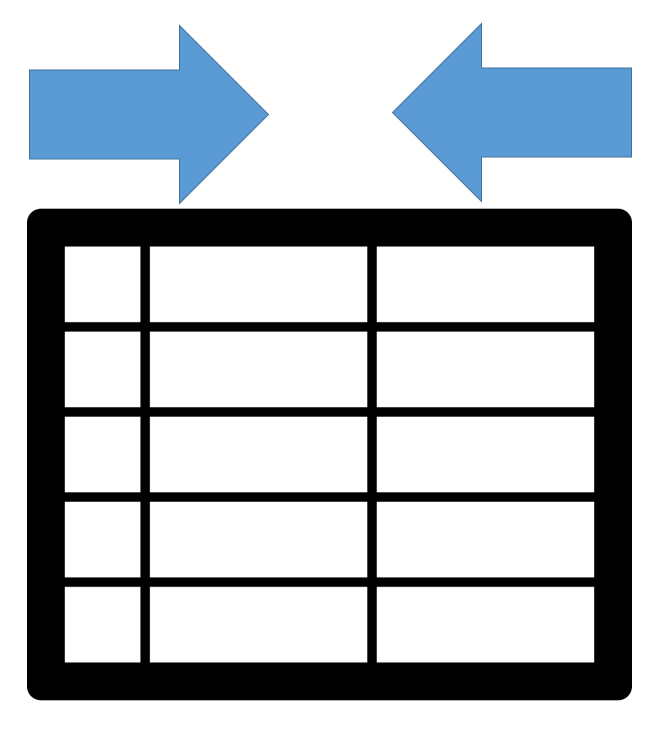
\includegraphics{src/images/dimreduce}}
    \caption{Horizontal Data Reduction}
    \label{fig:my_label}
\end{figure}

\begin{figure}[H]
    \centering
        \scalebox{.1}{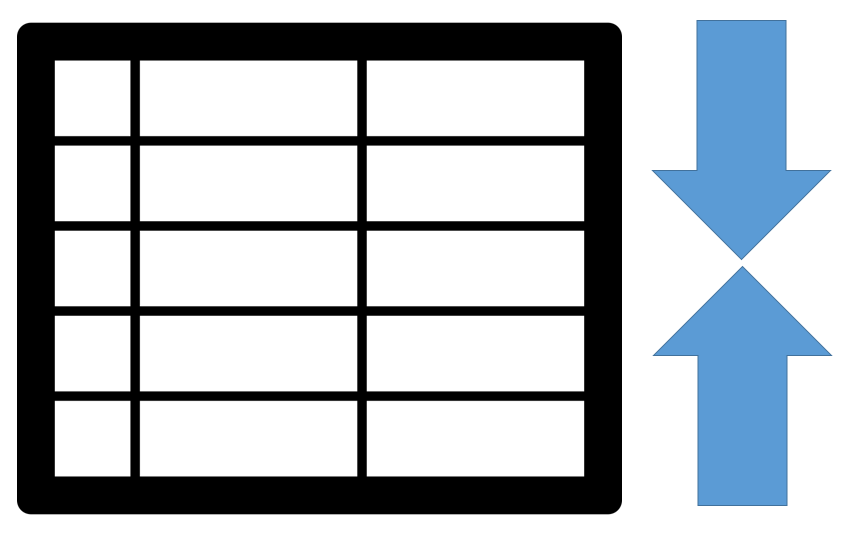
\includegraphics{src/images/aggregation}}
    \caption{Vertical Data Reduction}
    \label{fig:my_label}
\end{figure}

\subsection{Vertical Data Reduction}
One way to decrease the size of large or huge data sets is to remove data rows. This section lists several data removal techniques. One important issue for every technique is the question which data to keep and which data to remove. The disadvantage of data reduction is the information loss.
\subsubsection*{Sampling}
Sampling describes a strategy to reduce data by creating a sample of the original data. Thereby, sampling is scalable, reduces clutter, preserves information of the kept data as well as patterns and trends\cite{PiringerHarald2011}. Still, sampling may eliminate outliers or single data items and does not provide any garantuee to avoid visual overlap. 
\subsubsection*{Filtering}
Filtering is a method to reduce data by some specific criteria. In visualization filtering often is based on user input such as dynamic query sliders. Thereby, filtering can support the user in excluding task-irrelevant data portions and unlike sampling filtering may be appropriate to detect outliers. However, as filtering is based on the exlusion of unrelevant attributes it does not garantuee a specific target size of the data set. In some cases the target size might still be too large. Moreover, filtering also does not garantuee to discriminate distinct data items\cite{PiringerHarald2011}.
\subsubsection*{Temporal Data Abstraction}
Temporal Data Abstraction\cite{Aigner2011} reduces the number of data rows by focusing on relevant concepts, patterns, shapes over time and neglecting irrelevant details. Clusters and summery statistics\cite{PiringerHarald2011} are typical examples for data abstraction. However, the authors found a trade-off between abstraction and accuracy: with low abstraction and a high accuracy there exists the problem of cluttering. \todo{besser integrieren}
One way to implement temporal data abstraction is to use natural language processing in visualization tools. \todo{wie formuliere ich das am besten? Answerrocket + google}
Clustering as defined in the user tasks~\ref{sec:user} have the advantage of reducing visual clutter by displaying the natural groups of the data instead of every single data item. Clustering has the advantage of pattern and outlier preservation if the similarity measure is appropriate.
\subsubsection*{Aggregation}
Aggregation describes the process of grouping several data items together. Hierarchical aggregation builds aggregated data items by forming a tree structure and collapsing the children of a tree\cite{elmqvist2010hierarchical}. Binned aggregation devides data into adjacent bins and combines them for aggregation\cite{Liu2013}. Pixel-aware aggregation clusters pixels according to their screen coordinates\cite{li2016polyspector}. M4 aggregation compresses time series data into a set of equidistant time spans\cite{jugel2014m4}.
As time-oriented data has specific characteristics analytical methods have to consider these peculiarities. One way to reduce data size with respect to the time-specific characteristics is temporal aggregation. Hereby, data is aggregated according to the time unit (day, month, year) in temporal hierarchy levels. Examples for temporal aggregation are hierarchical axis \cite{Chung2014} which enable to navigate in time. \todo{mich damit beschäftigen}
\\*
Other ways to reduce data vertically are binning and pivotization. We will not explain them here in detail as they treat continuous and hierarchical datasets which are beyond our scope in this work. 

\subsection{Horizontal Data Reduction}
Besides data removal datasize can be reduced by decreasing data dimensionality. Since business data often is multi-dimensional but visualization techniques are limited in the number of attributes dimensionality reduction is a way to process data sets in a way that they can be displayed by visualization techniques. A common way to map a high-dimensional to a low dimensional space is the Principal Component Analysis (PCA)\cite{Aigner2008}. Other approaches are Multi-Dimensional Scaling or Self-Organizing Maps\cite{PiringerHarald2011}. The advantage is that they keep similarities after the projection. However, the attributes in the low-dimensional space are difficult to understand which makes them unintuitive. To overcome this problem hierarchical dimension reduction has been proposed. \todo{Quellen einfügen + evtl. ausformulieren}
%Segmentation Techniques, Factor Analysis, Multidimensional Scaling, FastMap\cite{FerreiradeOliveira2003} Correlation analysis, Information gain or Statistical methods, Sampling, Clustering or Aggregation\cite{Keim2005}



% 3 Methods for Large Data (Aigner2008)
% 1. Temporal Data Abstraction: VIE-VENT + The Spread
% 2. Data Abstraction for Multivariate Data: PCA
% 3. Data Aggregation




Moreover, besides the database metrics and the visualization characteristic visual scalability is influenced by six factors: 
\begin{itemize}
    \item Human Perception\cite{Keim2005,Deering1998}
    \item Monitor Resolution 
    \item Visual Metaphors
    \item Interactivity
    \item Data structures and algorithms
    \item Computational infrastructure
\end{itemize}
\todo{Entscheiden, inwiefern ich diese 6 Faktoren mit aufnehme. Wenn ich sie mit aufnehme, muss ich sie auch erläutern}

\subsubsection*{Human Perception} 
% What can humans perceive? How many pixels? 
One way to measure the viual ability to see details is called \textit{visual acuity}\cite{Ware2012a}. 
According to experiments discussing the limits of human perception \cite{Deering1998} the human visual system is able to perceive 15mio pixels per eye. Assuming that the amount of perceivable pixels for two eyes is larger than 15mio pixels but smaller than 30mio pixels due to the overlap of the field of view the max. amount of perceivable pixels (pp) is:
\begin{math}
15 mio. \leq pp < 30 mio.
\end{math}
Nevertheless, the important question is not the amount of perceivable pixels but whether the data structure, patterns, trends and further information in the data can be perceived. To achieve this goal Keim\cite{Keim2005} created \textit{CircleView}.
%Talking of scalability visualization techniques should be able to scale according to their data types, data sources and levels of quality \cite{Keim2008}. 
\subsubsection*{Focal Depth-of-Focus Information}
\\*
\subsubsection*{Monitor Resolution}
Even though large wall-sized screens have been developed in business usually. \todo{schreiben}
\\*
\subsubsection*{Visual Metaphors}
Improved visual metaphors enhance the scalability of visualization techniques\cite{Eick2002}. \todo{Beispiel} One way to improve visual metaphors are multi-resolution metaphors\cite{Keim2005}. These show less details at the \textit{Overview-Level} of a visualization and more details at the \textit{Detail-Level}. \textit{CircleView} is one visualization technique with a multi-resolution metaphor which clusters data items according to their relevance and displays the clusters first.
\\*

\textbf{Pixel-oriented} techniques map a data point to a colored pixel. Since each data entry requires one pixel on the monitor pixel-based visualizations can maximal display around 2.000.000. data points. Moreover, they use multiple windows and center the most relevant data in the middle and the less relevant data outside the center\cite{Keim1996}.\\*


\section{Parameterization}

\section{Need for Interaction Techniques}
Interaction Techniques describe how the user can interact with the data. As interaction is a crucial factor for scalable visualization techniques it enhances visual scalability\cite{tegarden1999}. 
Hereby, we assume that interaction is in responsibility of the visualization tools. Keim\cite{2002} devided interaction techniques into two classes of techniques. The first group supports the user in exploring the data \textit{interaction techniques} and the second helps in displaying large databases \textit{distortion techniques}. \\*
\textbf{Interaction techniques} include several techniques such as dynamic projection, filtering, zooming, and linking \& brushing.
The main idea of \textbf{interactive distortion techniques} is the presentation of showing the data at different levels of detail. Examples are hyberbolic and spherical distortion, bifocal displays, perspective wall, graphical fisheye view, hyperbolic visualization and hyperbox\cite{Keim2002}\todo{genauere Zitierung}. 

\subsubsection*{Filtering}

\subsubsection*{Selecting}
Selecting of a single data item or a range of data items.
\subsubsection*{Linking}
Linking describes the connection between multiple views. \textit{Linking} in the context of large data is important to provide overview and detail views. 
\textbf{Brushing \& Linking}\\*
The user can select data items on the screen(Brushing) and the respective items are highlighted in every connected window (Linking). Therefore, lasso, rubber-band or rectangular selection enables the user to select groups of data items\cite{tegarden1999, Aigner2011}. In the context of time-oriented data a typical brushing activity is the selection of an smaller time-span to see more details during this period of time.
\textbf{Dynamic Queries}\\*
Besides Brushing \& Linking, dynamic queries provide a filter-mechanism by multiple widgets, such as sliders or input fields\cite{Hochheiser2004,Shneiderman2008,Aigner2011}. A specific dynamic query are time-boxes. These boxes are rectangular selection areas which are drawn by the user. The tool then only displays values with a similar pattern to the pattern in the time-boxes.
\textbf{Focus + Context} shows a selected region of interest in detail while the rest of the dataset is still shown\cite{Keim2005}. 
\textbf{Drill down}
\textbf{Fish-eye Views}\\*
\textbf{Table Lens}\\*
\textbf{Magic Lense}\\*
\textbf{Perspective walls\cite{Keim2005}}\\*
\textbf{Zoom + Filter}\\*



\subsection{Advanced Interaction Techniques}
\textbf{Navigation Maps}\\*
For navigating through massive datasets 
\textbf{Information Mural}
\textbf{Coarse Presentations}

\section{Layout}
Closely related to interaction techniques is an appropriate layout to enhance visual scalability. Ware\cite{Ware2012} showed that zooming is an easy-to-use-tool for a small amount of items. However, if the user needs to keep three items or more in its visual working memory multiple windows are more effective than zooming. Thus, displaying large time-oriented requires a layout with multiple simultaneous views. Coordinated views are linked views. If one data item is selected and brushed the corresponding characteristic in other windows is also highlighted.
\begin{figure}[H]
    \centering
        \scalebox{.3}{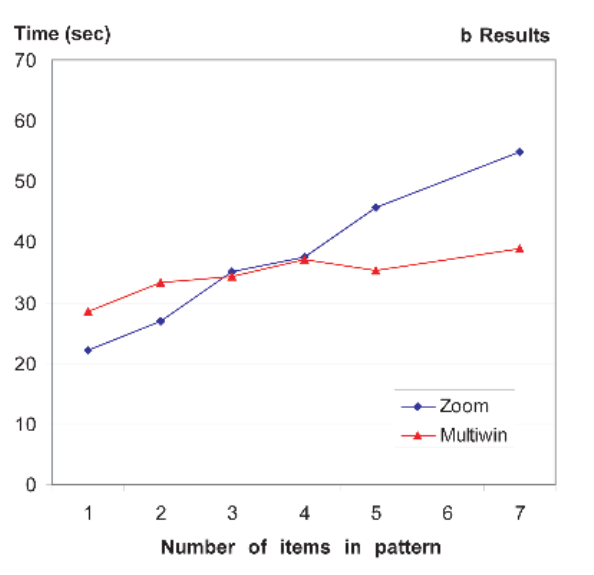
\includegraphics{src/images/zoomVSmultiWindow}}
    \caption{Measured task performance of zooming compared to multiple windows. \cite{Ware2012a}}
    \label{fig:my_label}
\end{figure}
Other techniques are \textit{distortion techniques}\cite{mackinlay1991perspective}: \textit{Bifocal Displays}\cite{Spence1982}, \textit{Perspective Walls}\cite{mackinlay1991perspective}